\documentclass[11pt,a4paper]{article}

\usepackage[T1]{fontenc}
\usepackage[utf8]{inputenc}
\usepackage[margin=0.85in]{geometry}
\usepackage{amsmath,amssymb,bm}
\usepackage{booktabs}
\usepackage{array}
\usepackage{graphicx}
\usepackage{caption}
\usepackage{xcolor}
\usepackage{hyperref}
\usepackage{listings}
\usepackage{tikz}
\usetikzlibrary{arrows.meta,positioning,fit}

\hypersetup{
  colorlinks=true,
  linkcolor=blue!55!black,
  urlcolor=blue!55!black,
  citecolor=blue!55!black
}

\graphicspath{{./}{report_figures/}{logs/plots/}}
\lstset{
  basicstyle=\ttfamily\small,
  breaklines=true,
  breakatwhitespace=true,
  columns=fullflexible,
  frame=single,
  xleftmargin=0.5em,
  xrightmargin=0.5em
}

\newcommand{\state}{\bm{x}}
\newcommand{\meas}{\bm{z}}
\newcommand{\prior}{\state_k^-}
\newcommand{\post}{\state_k^+}
\newcommand{\gain}{K}
\newcommand{\trust}{\bm{\gamma}}
\newcommand{\avail}{\bm{a}}
\newcommand{\innov}{\bm{r}}
\newcommand{\wrap}{\operatorname{wrap}}
\newcommand{\diag}{\operatorname{diag}}

\title{\vspace{-1em}Robust Gamma-KalmaNet State Estimation for QCar}
\author{Quang Huy Nugyen \and Echrak Chnib}

\date{\today}

\begin{document}
\maketitle

\begin{abstract}
This report summarizes the robust KalmaNet/RKNet estimator developed for the
QCar platform. The estimator keeps the QCar physical prediction model and
learns the uncertain part of the filter: how much each measurement should be
trusted and how strongly the state should be corrected. In this report the
learned measurement trust vector is denoted by $\trust_k$ and is treated as the
``robust gamma'' gate. The current implementation estimates
$\state=[x,y,\psi,v]^T$ from GPS position, fused heading, tachometer velocity,
IMU, steering, and wheel speed signals. Training uses real QCar logs together
with synthetic GPS, heading, velocity, IMU, steering, and wheel-speed attacks.
The saved training history shows a large reduction in attacked validation loss:
from 1.1095 at the first logged epoch to 0.4028 at the best robust checkpoint.
Offline validation on a separate dataset also shows lower four-state RMSE for
the learned estimator than the kinematic reference. The main conclusion is that
the method is not a pure black-box neural estimator; it is a hybrid filter where
vehicle physics gives the prior and the recurrent neural update learns when to
reject corrupted measurements.
\end{abstract}

\section{Introduction}

Autonomous QCar experiments require a state estimate that is accurate enough
for feedback control and stable enough during bad sensor periods. A standard
Extended Kalman Filter (EKF) is a strong baseline when its assumptions are
correct. It uses a vehicle model for prediction and a measurement model for
correction. However, the EKF can become fragile when the measurement noise is
not just random noise but a structured fault: GPS jumps, GPS dropout, frozen
velocity, wheel speed scaling, heading glitches, or short IMU bursts. In those
cases the filter may apply a correction in the wrong direction because the
measurement is still treated as believable.

The work in this folder builds a robust KalmaNet-style estimator for the QCar.
The key design choice is simple:
\begin{quote}
  keep the vehicle model for prediction, and learn a trust-controlled update
  for difficult sensor behavior.
\end{quote}
The learned trust vector $\trust_k$ is the important element. When a channel is
clean, its trust should stay high. When a channel is attacked or unavailable,
its trust should decrease so that the innovation cannot force a large state
jump. This is close in spirit to KalmanNet \cite{revach2022kalmannet} and
RobustStateNet \cite{dahal2024robuststatenet}, but the current QCar
implementation is more conservative: the prediction step is currently an
analytical QCar bicycle model, not a learned predictor.

\section{Problem Definition}

\subsection{State and Measurement}

The active training and runtime state is
\begin{equation}
  \state_k =
  \begin{bmatrix}
    x_k & y_k & \psi_k & v_k
  \end{bmatrix}^{T},
\end{equation}
where $x$ and $y$ are global position, $\psi$ is heading, and $v$ is forward
velocity. Some older recorded files contain a fifth yaw-rate channel, but the
current robust KalmaNet configuration slices the target and measurement arrays
to the first four states.

The measurement vector is
\begin{equation}
  \meas_k =
  \begin{bmatrix}
    x_{gps,k} & y_{gps,k} & \psi_{fused,k} & v_{tach,k}
  \end{bmatrix}^{T},
  \qquad
  \meas_k = H\state_k + \bm{n}_k,
  \qquad
  H \approx I_4 .
\end{equation}
The measured heading is rebuilt offline using the same QCar heading-fusion path
used by the local estimator. GPS metadata is kept because it is essential to
separate real measurement faults from normal innovation.

\subsection{Raw Sensor Inputs}

The model receives raw inputs grouped by physical source:
\begin{itemize}
  \item IMU branch: velocity context, heading context, acceleration, and yaw
  rate;
  \item steering branch: velocity context, heading context, and steering angle;
  \item wheel branch: velocity context, heading context, and four wheel-speed
  channels;
  \item availability metadata: GPS valid flag, heading valid flag, GPS hold
  flag, and GPS age.
\end{itemize}

This separation matters because each sensor family has different failure
behavior. GPS position can jump or disappear. Velocity can freeze or become
scaled. IMU signals can become noisy or biased. The learned update uses these
signals to decide whether the current measurement should be trusted.

\section{Estimator Architecture}

Figure~\ref{fig:architecture} shows the estimator at a high level. The
prediction side is deterministic. The update side is learned and recurrent.

\begin{figure}[htbp]
\centering
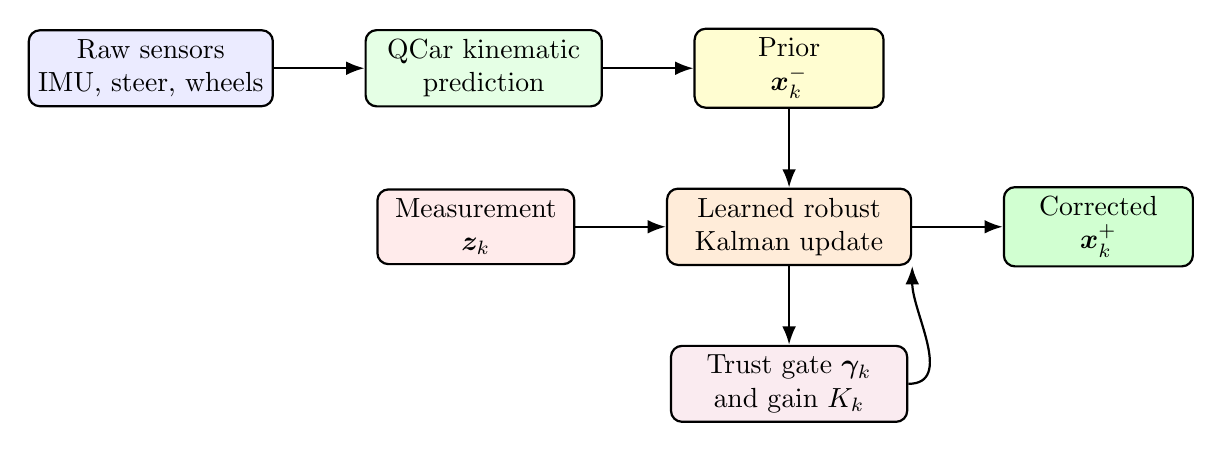
\begin{tikzpicture}[node distance=1.0cm and 1.15cm,>=Latex,thick]
  \node[draw,rounded corners,align=center,fill=blue!8,
        minimum width=2.8cm,minimum height=0.9cm] (raw)
        {Raw sensors\\IMU, steer, wheels};
  \node[draw,rounded corners,right=of raw,align=center,fill=green!10,
        minimum width=3.0cm,minimum height=0.9cm] (pred)
        {QCar kinematic\\prediction};
  \node[draw,rounded corners,right=of pred,align=center,fill=yellow!18,
        minimum width=2.4cm,minimum height=0.9cm] (xp)
        {Prior\\$\prior$};
  \node[draw,rounded corners,below=1.0cm of xp,align=center,fill=orange!15,
        minimum width=3.1cm,minimum height=0.9cm] (upd)
        {Learned robust\\Kalman update};
  \node[draw,rounded corners,left=of upd,align=center,fill=red!8,
        minimum width=2.5cm,minimum height=0.9cm] (z)
        {Measurement\\$\meas_k$};
  \node[draw,rounded corners,right=of upd,align=center,fill=green!18,
        minimum width=2.4cm,minimum height=0.9cm] (xu)
        {Corrected\\$\post$};
  \node[draw,rounded corners,below=of upd,align=center,fill=purple!8,
        minimum width=3.0cm,minimum height=0.8cm] (trust)
        {Trust gate $\trust_k$\\and gain $K_k$};

  \draw[->] (raw) -- (pred);
  \draw[->] (pred) -- (xp);
  \draw[->] (xp) -- (upd);
  \draw[->] (z) -- (upd);
  \draw[->] (upd) -- (xu);
  \draw[->] (upd) -- (trust);
  \draw[->] (trust.east) to[out=0,in=-90] (upd.south east);
\end{tikzpicture}
\caption{Hybrid RKNet structure used in this work. The prior is generated by
QCar physics. The neural update learns a measurement trust gate and a
Kalman-style gain.}
\label{fig:architecture}
\end{figure}

\subsection{Kinematic Prediction}

The active configuration uses \texttt{predictor\_mode: kinematic}. The
prediction step has no learned parameters. It is a bicycle-model update with
wheelbase $L$:
\begin{equation}
  \dot{\psi}_k =
  \frac{v_k\tan(\delta_k)}{L},
\end{equation}
where $\delta_k$ is the steering angle. The predicted pose is
\begin{align}
  x_k^- &= x_{k-1}^+ + v_{pose,k}\cos(\psi_{k-1}^+)\Delta t, \\
  y_k^- &= y_{k-1}^+ + v_{pose,k}\sin(\psi_{k-1}^+)\Delta t, \\
  \psi_k^- &=
  \wrap\left(\psi_{k-1}^+
  + \frac{v_{pose,k}\tan(\delta_k)}{L}\Delta t\right).
\end{align}

The active velocity model is \texttt{velocity\_lag}. It predicts velocity from
the previous velocity and throttle:
\begin{equation}
  \dot{v}_k =
  \frac{-v_{k-1}^+ + g u_k}{\tau},
  \qquad
  v_k^- =
  \operatorname{clip}\left(v_{k-1}^+ + \dot{v}_k\Delta t\right).
\end{equation}
The current values in \texttt{robust\_kalmannet\_train\_config.yaml} are
$L=0.2$, $\tau=0.301$, $g=6.598$, $|v|\leq2.0$ m/s, and maximum acceleration
$2.0$ m/s$^2$.

\subsection{Learned Robust Update}

The learned update receives the prior $\prior$, the previous corrected state
$\state_{k-1}^+$, the current measurement $\meas_k$, the previous measurement
$\meas_{k-1}$, and availability metadata. It forms three main residual terms:
\begin{align}
  \Delta \state_k &= \wrap(\state_k^- - \state_{k-1}^{+}), \\
  \innov_k &= \wrap(\meas_k - H\state_k^-), \\
  \Delta \meas_k &= \wrap(\meas_k - \meas_{k-1}).
\end{align}

The hard availability vector is
\begin{equation}
  \avail_k =
  \begin{bmatrix}
    g_k & g_k & h_k & 1
  \end{bmatrix}^{T},
\end{equation}
where $g_k$ is the GPS-position valid flag and $h_k$ is the heading valid flag.
Unavailable measurement channels are removed before the learned correction.

The update feature vector is
\begin{equation}
\begin{aligned}
  \bm{f}_k =
  [&\Delta\state_k / \bm{s}_x,\,
    (\avail_k \odot \innov_k) / \bm{s}_z,\,
    (\avail_k \odot \Delta\meas_k) / \bm{s}_z,\,
    \avail_k,\\
   &g^{hold}_k,\,
    \log(1+\min(age_k,10)),\,
    \log(1+|\avail_k\odot\innov_k|),\,
    \log(1+|\avail_k\odot\Delta\meas_k|)] .
\end{aligned}
\end{equation}
For the four-state model this gives a 26-dimensional update feature vector.
The scale vectors used by the active config are
\[
  \bm{s}_x=\bm{s}_z=[0.25,\ 0.25,\ 0.20,\ 0.50].
\]

The robust gamma/trust vector is generated by a small MLP:
\begin{equation}
  \trust_k = \sigma(MLP_{\gamma}(\bm{f}_k)).
\end{equation}
Only the measurement part of this vector is used directly as the measurement
trust gate. Clean channels should stay close to one; attacked channels should
move toward zero.

The Kalman-style gain is generated by a GRU and an MLP:
\begin{align}
  \bm{h}_k &= GRU(\trust_k \odot \bm{f}_k,\bm{h}_{k-1}), \\
  K_k &= s\tanh(MLP_K(\bm{h}_k)).
\end{align}
The current tanh scale is $s=1.2$. The implementation also applies exponential
smoothing to the gain and trust gate with $\alpha=0.35$.

The corrected state is
\begin{equation}
  \state_k^+
  =
  \state_k^-
  +
  K_k
  \left(
    \avail_k \odot \trust_k^z \odot \innov_k
  \right),
  \label{eq:robust_update}
\end{equation}
where $\trust_k^z$ is the measurement-trust part of the learned gate. Equation
\eqref{eq:robust_update} is the main robustness mechanism. A corrupted GPS or
velocity measurement may create a large innovation, but the innovation is first
multiplied by the learned trust gate before it reaches the gain. The runtime
also clamps the per-step correction to
\[
  [0.35,\ 0.35,\ 0.35,\ 0.80]
\]
for $[x,y,\psi,v]$.

\section{Dataset and Training}

\subsection{Recorded Dataset}

The dataset recorder saves time-aligned raw signals, measurement vectors,
target states, timestamps, and JSON metadata. The active training configuration
points to
\begin{center}
\texttt{datasets/robust\_kalmannet\_dataset\_V0\_20260417\_094048.npz}.
\end{center}
Its metadata reports 52,921 samples, 671.84 seconds of driving, and mean
timestep 0.0127 seconds. The target estimator type is EKF, so the supervised
target is a clean/reference estimator rather than motion-capture ground truth.

\begin{table}[htbp]
\centering
\caption{Main dataset and training configuration used by the saved model.}
\label{tab:dataset}
\begin{tabular}{ll}
\toprule
Item & Value \\
\midrule
State order & $[x,y,\psi,v]$ \\
Measurement order & $[x_{gps},y_{gps},\psi_{fused},v_{tach}]$ \\
Active dataset & \texttt{V0\_20260417\_094048.npz} \\
Samples / duration & 52,921 samples / 671.84 s \\
Mean timestep & 0.0127 s \\
Validation split & final 20\% of sequence \\
Training windows & $T=50$ for Phase B, $T=80$ for Phase C \\
Predictor mode & kinematic QCar bicycle model \\
Updater hidden size & 32 \\
Gain hidden size & 32 \\
Optimizer learning rate & $1.0\times10^{-4}$ \\
\bottomrule
\end{tabular}
\end{table}

\subsection{Training Phases}

The code supports a learned predictor, but the active predictor is kinematic.
Therefore predictor pretraining is automatically skipped. The useful phases are:
\begin{itemize}
  \item Phase B: freeze the predictor and train only the learned updater;
  \item Phase C: fine tune the complete recurrent runtime loop with teacher
  forcing disabled.
\end{itemize}

The state loss is weighted MSE:
\begin{equation}
  L_{state}
  =
  \frac{1}{N}\sum_k
  \left\|
  W^{1/2}(\hat{\state}_k-\state_k^\star)
  \right\|_2^2,
  \qquad
  W=[1.0,\ 1.0,\ 2.5,\ 1.2].
\end{equation}

The full loss combines state accuracy, trust supervision, gain regularization,
and temporal smoothness:
\begin{equation}
\begin{aligned}
  \mathcal{L}
  &=
  \lambda_u L_{upd}
  + \lambda_p L_{pred}
  + \lambda_{\gamma} L_{\gamma}
  + \lambda_K L_K
  + \lambda_{\Delta K} L_{\Delta K}
  + \lambda_{\Delta\gamma} L_{\Delta\gamma}.
\end{aligned}
\end{equation}
The active Phase C weights are $\lambda_u=0.85$ and $\lambda_p=0.15$.
Measurement-mask supervision uses a clean target of one and an attacked target
of zero for each affected measurement channel.

\section{Sensor Attack Augmentation}

The training data is not only clean driving. Synthetic attacks are injected
offline so the model sees examples of sensor faults and receives supervision
for which channels should be trusted.

\begin{table}[htbp]
\centering
\caption{Active augmentation configuration.}
\label{tab:augmentation}
\begin{tabular}{lll}
\toprule
Attack group & Probability & Enabled failure types \\
\midrule
Raw branch attack & 0.25 & bias, scale, freeze, noise, ramp, zero-out \\
Direct measurement attack & 0.35 & heading and velocity corruption \\
GPS position attack & 0.45 & noise, freeze, jump, dropout, reacquisition \\
Maximum raw branches attacked & 1 & one of IMU, steering, wheel \\
\bottomrule
\end{tabular}
\end{table}

The GPS attacks are especially important for QCar because GPS position directly
drives $x$ and $y$ correction. A jump attack can make the EKF snap to a wrong
position unless the measurement is down-weighted. A dropout attack is different:
the availability gate should remove $x/y$, while the learned update continues
using the remaining channels.

\section{Results}

\subsection{Training History}

The saved file \texttt{models/robust\_kalmannet.train\_history.json} contains
20 logged epochs after Phase A was skipped. The best robust checkpoint was
selected at epoch 15 in Phase B. Table~\ref{tab:train_result} summarizes the
main points.

\begin{table}[htbp]
\centering
\caption{Saved training history. Selection loss combines clean and attacked
validation, with attacked validation weighted more strongly.}
\label{tab:train_result}
\begin{tabular}{lcccc}
\toprule
Checkpoint point & Epoch & Clean val. & Attacked val. & Selection loss \\
\midrule
First logged epoch & 1 & 0.00668 & 1.10951 & 0.66838 \\
Best robust checkpoint & 15 & 0.01751 & 0.40279 & 0.24868 \\
Final Phase C checkpoint & 20 & 0.02408 & 0.43457 & 0.27037 \\
\bottomrule
\end{tabular}
\end{table}

The attacked validation loss decreases from 1.10951 to 0.40279 at the selected
best robust checkpoint, a reduction of about 63.7\%. The clean validation loss
is higher at the robust checkpoint than at the first clean-only epoch. This is
an expected tradeoff: the estimator becomes more conservative so it can survive
corrupted measurements.

\subsection{Offline Validation}

The validation script compares a kinematic reference and the learned RKNet
checkpoint against the saved EKF target. The file
\texttt{logs/validation/validation\_metrics\_best.json} reports the following
result on \texttt{V0\_20260401\_170829.npz}. Older validation files contain an
extra yaw-rate channel, so Table~\ref{tab:offline_rmse} reports only the active
four-state surface.

\begin{table}[htbp]
\centering
\caption{Offline RMSE against the EKF target on the best validation file.}
\label{tab:offline_rmse}
\begin{tabular}{lccccc}
\toprule
Method & $x$ [m] & $y$ [m] & $\psi$ [rad] & $v$ [m/s] & Mean, four states \\
\midrule
Kinematic reference & 0.0663 & 0.0574 & 0.1151 & 0.0134 & 0.0631 \\
Learned RKNet & 0.0076 & 0.0168 & 0.1096 & 0.0124 & 0.0366 \\
\bottomrule
\end{tabular}
\end{table}

The learned estimator strongly improves $x$ and $y$ RMSE and gives a smaller
four-state mean RMSE. Heading remains the hardest channel. This is reasonable
because heading is affected by angle wrapping, GPS heading availability, and
the reference itself.

\subsection{Runtime Comparator Run}

The latest plotted workspace summary used in this report is
\texttt{rknet\_workspace\_20260503\_025905}. It contains 8,413 model samples
over 95.97 seconds, with no fallback samples. It includes five attack segments
and 1,510 attack-active samples. Only 421 samples had fresh GPS, while 8,380
used GPS hold validity, so this run is useful for checking robustness during
limited fresh GPS availability.

\begin{figure}[htbp]
\centering
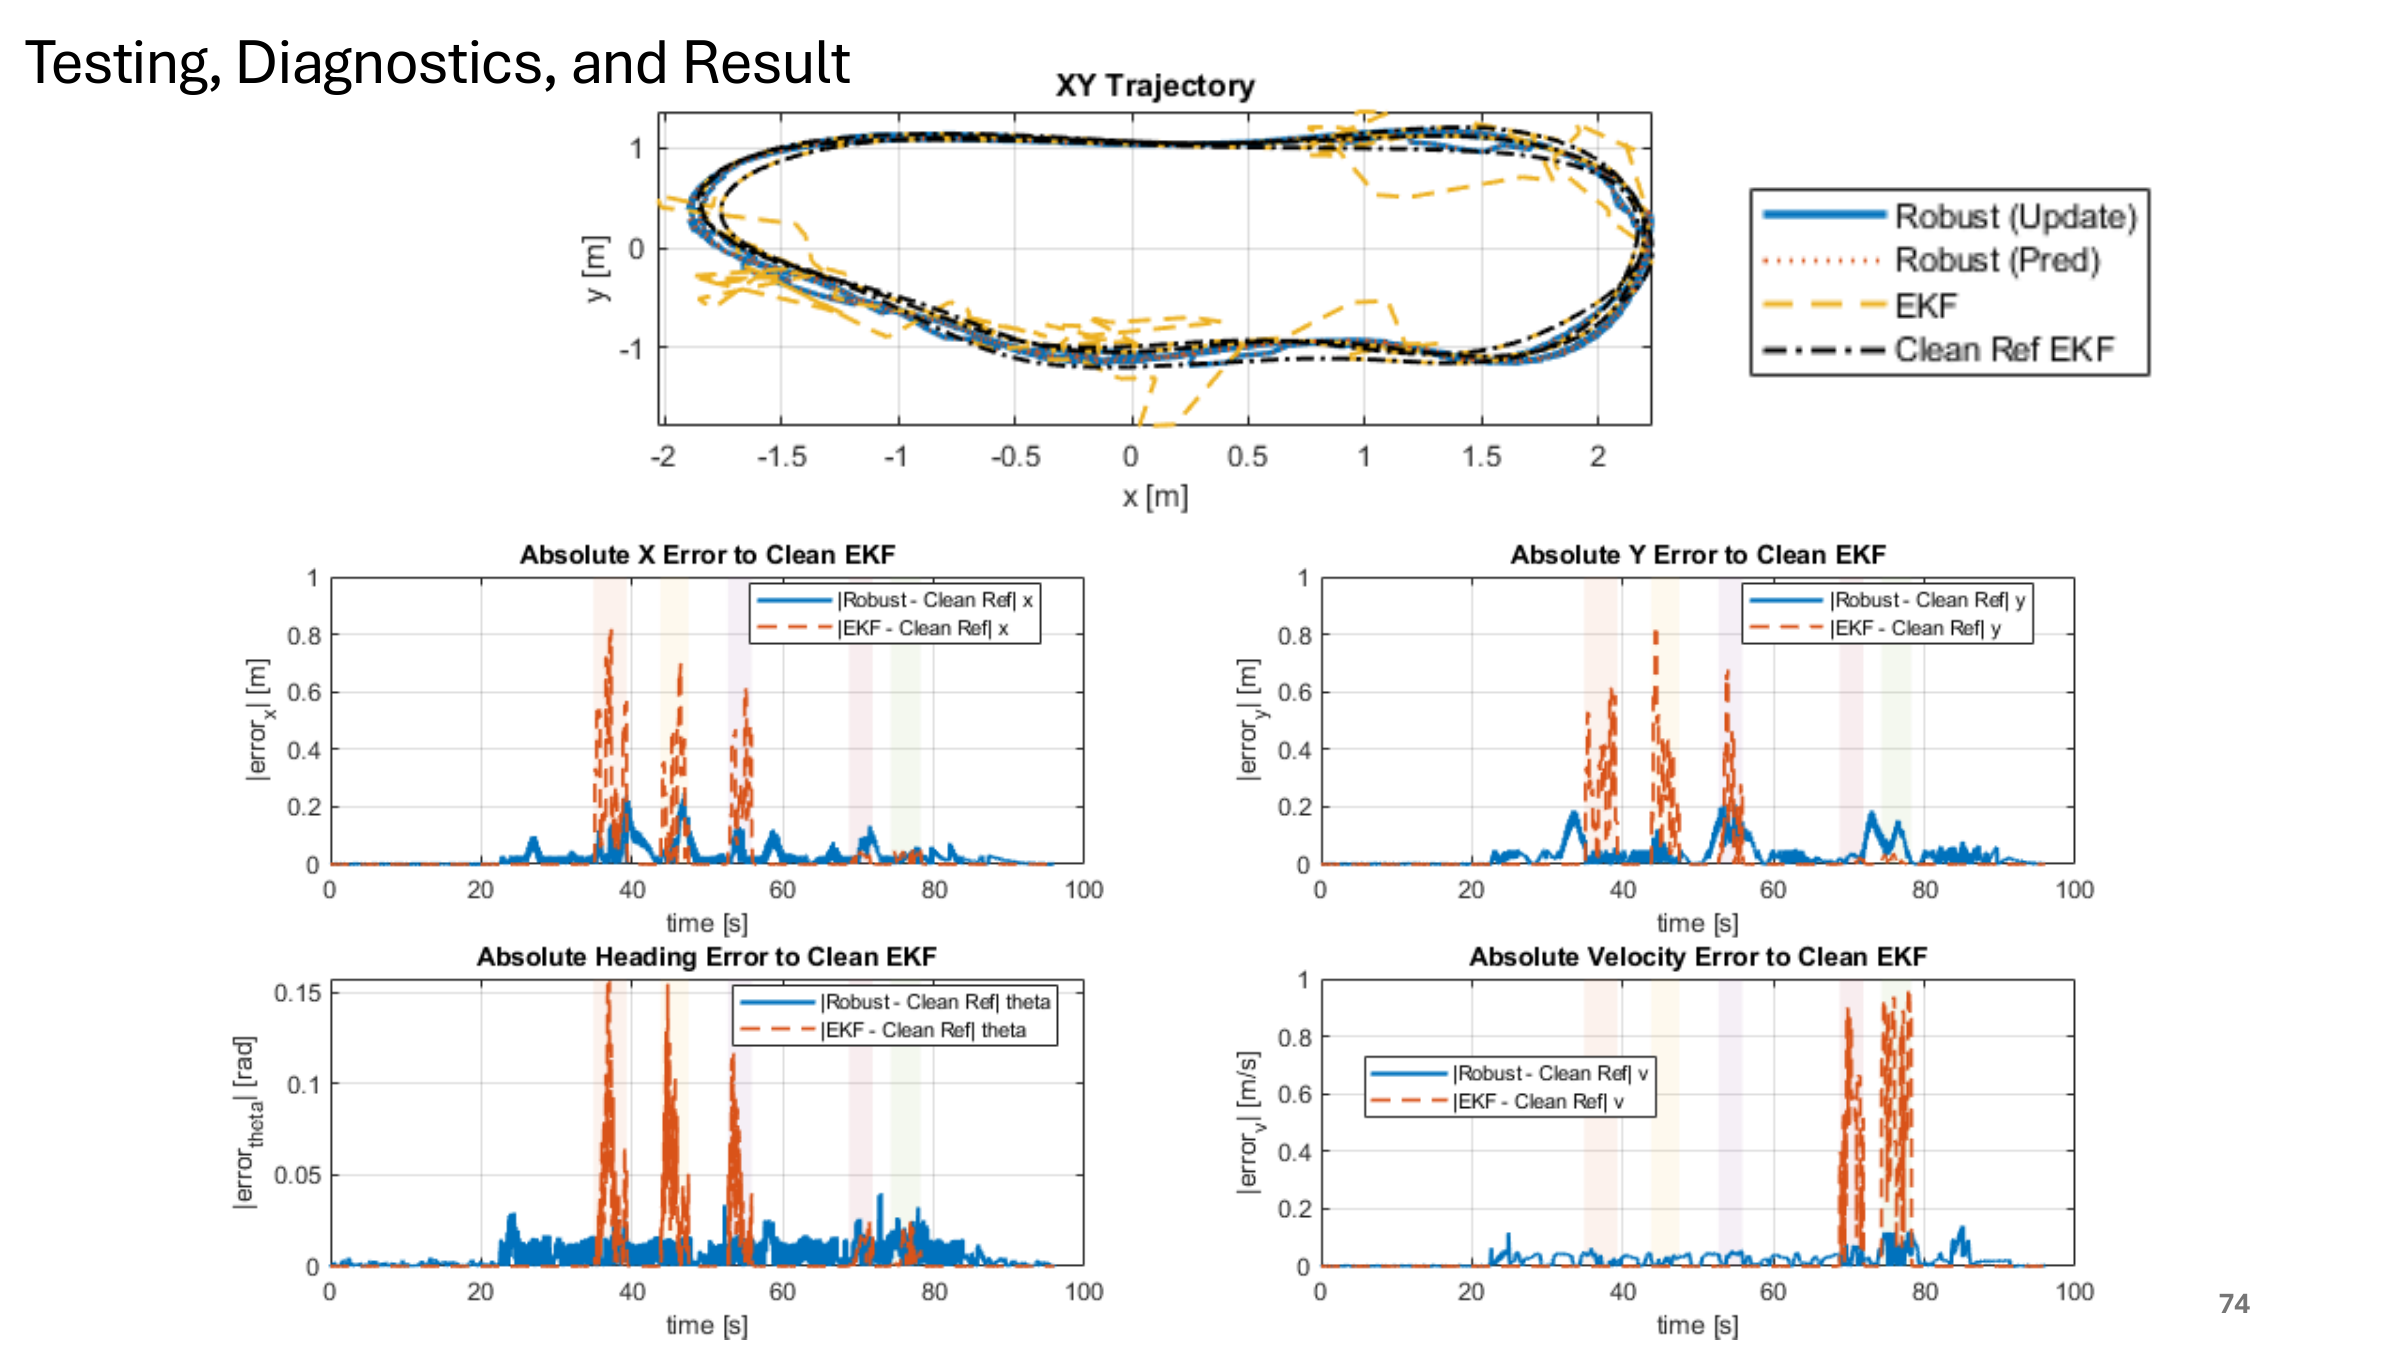
\includegraphics[width=0.98\linewidth]{kalmarobust_result-12.png}
\caption{Result figure rendered from \texttt{KalmaRobust\_Net\_Huy.pdf}. The
robust estimator follows the clean-reference EKF while the ordinary EKF shows
larger spikes during attack intervals.}
\label{fig:pdf_result_state}
\end{figure}

\clearpage

\begin{figure}[htbp]
\centering
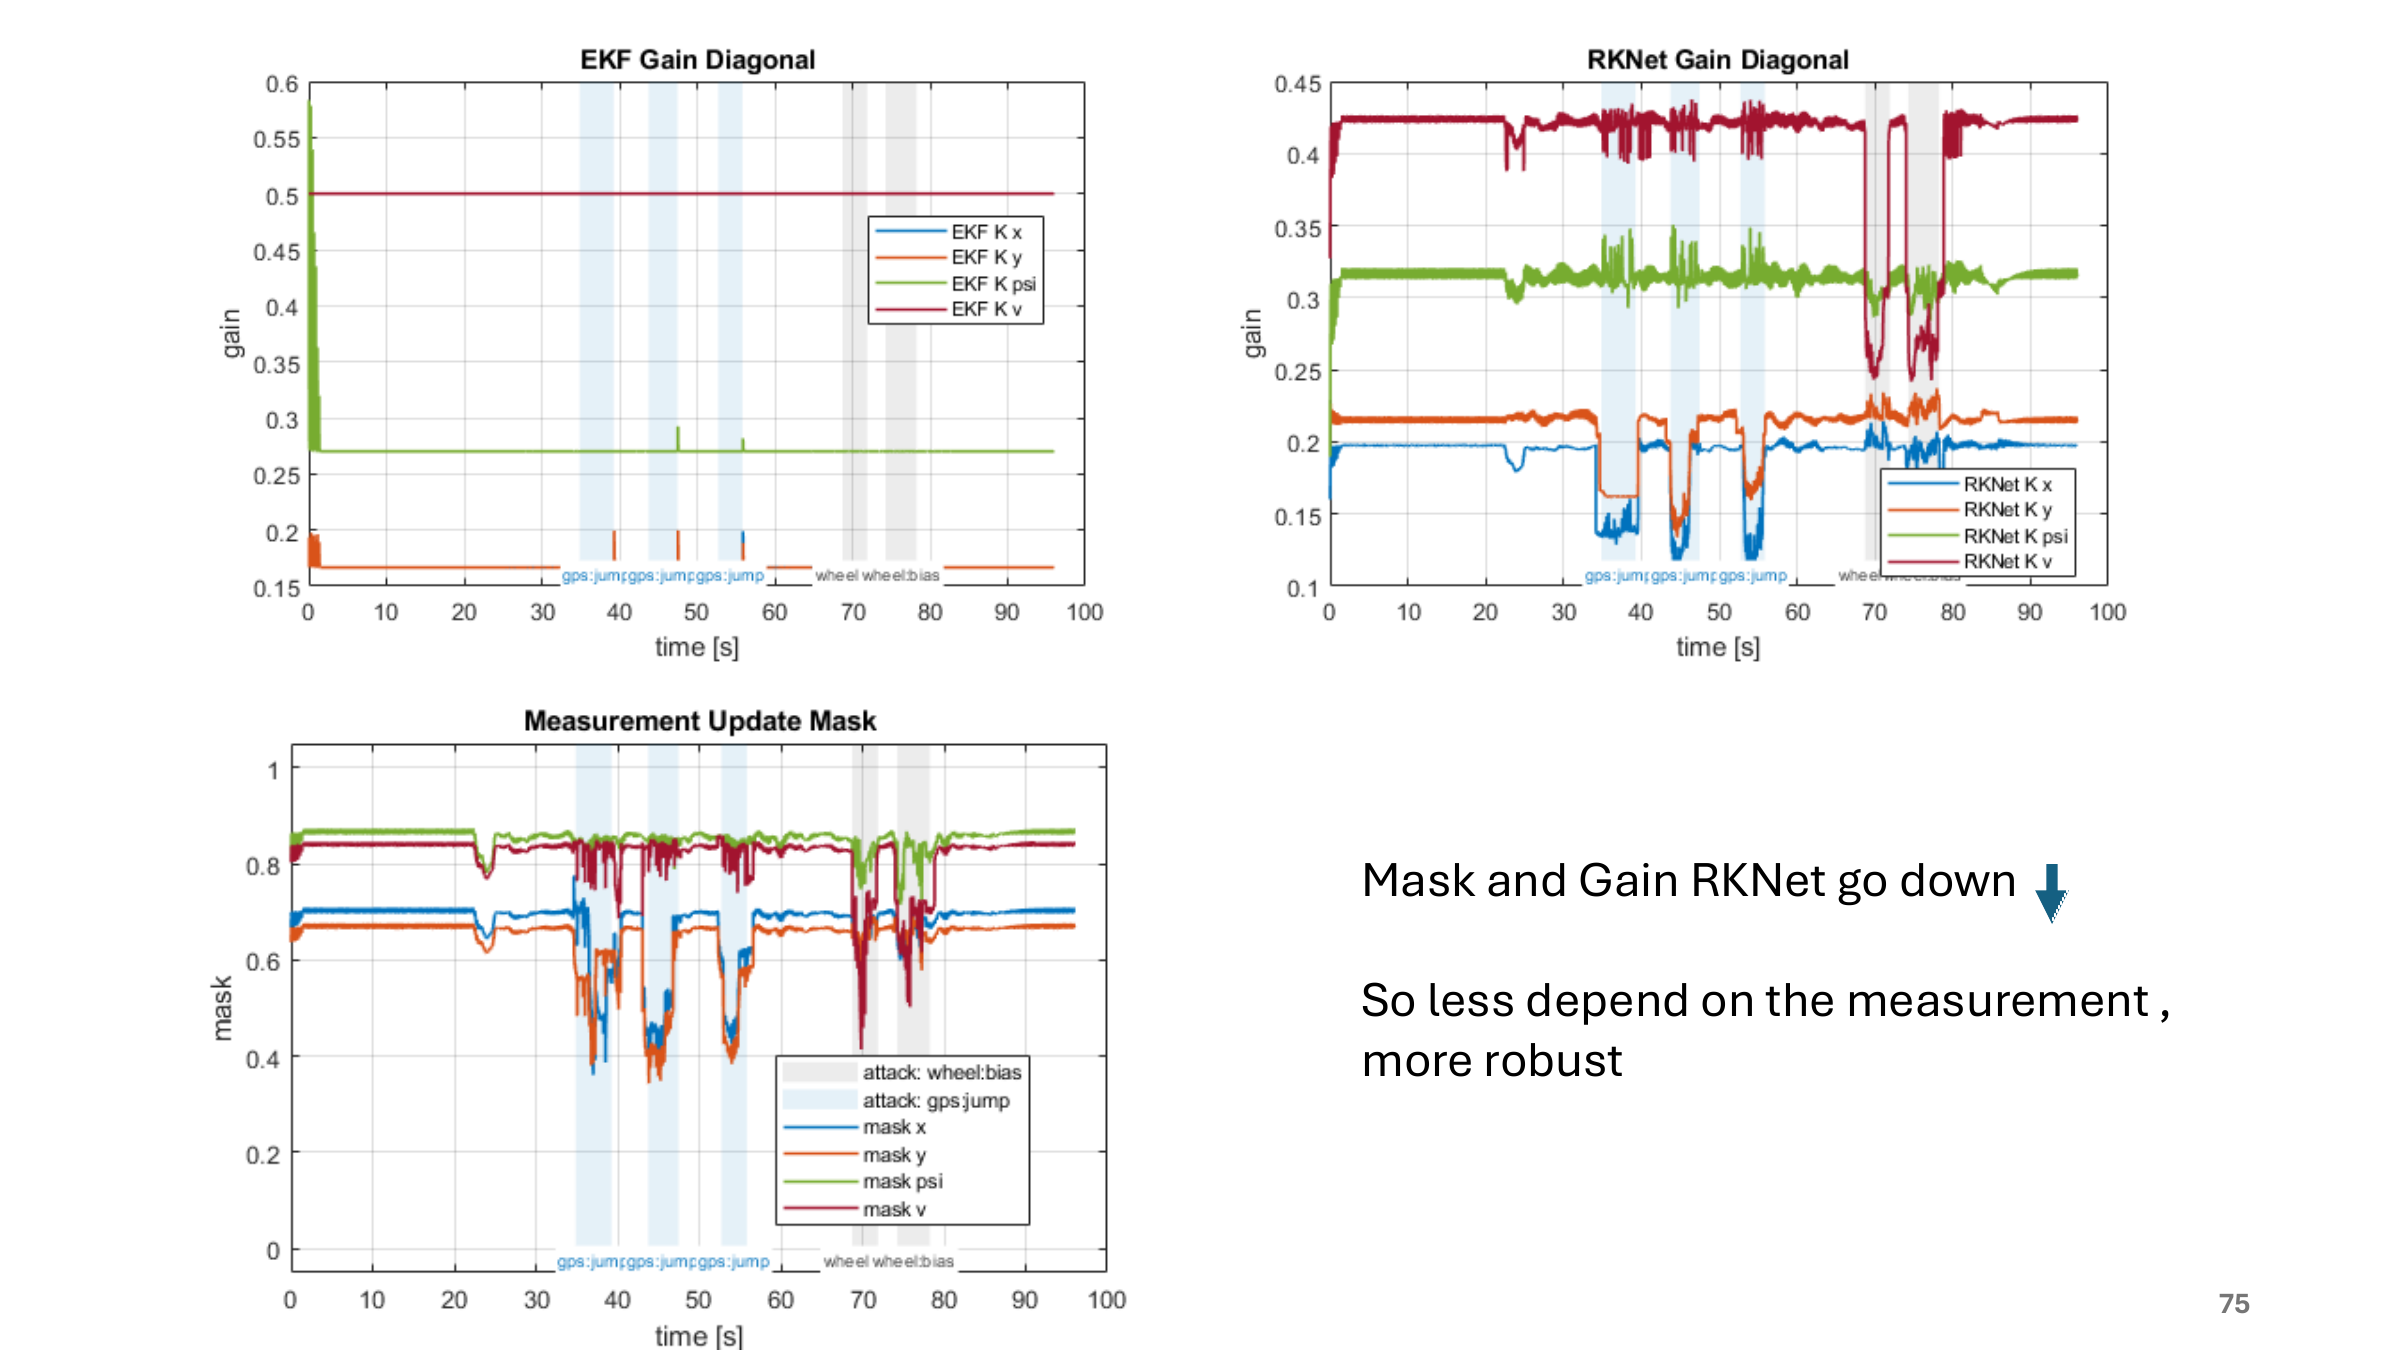
\includegraphics[width=0.98\linewidth]{kalmarobust_result-13.png}
\caption{Gain and measurement-mask behavior rendered from
\texttt{KalmaRobust\_Net\_Huy.pdf}. The learned mask and effective gain decrease
during GPS jump and wheel-bias intervals, reducing dependence on corrupted
measurements.}
\label{fig:pdf_result_mask}
\end{figure}

Figures~\ref{fig:pdf_result_state} and~\ref{fig:pdf_result_mask} show the main
behavior expected from the robust gamma gate. During the GPS jump intervals,
the measurement mask for position decreases and the effective diagonal gain
also drops. During wheel-bias intervals, the velocity-side trust and gain become
more conservative. This means the update is not blindly following the
measurement; it is using the innovation only after passing it through the
learned reliability gate.

\section{Discussion}

The important engineering result is the separation of responsibilities.
The QCar prediction step carries the vehicle kinematics and basic longitudinal
behavior. The neural update does not need to relearn the full vehicle model.
Instead, it learns the part that is hard to tune manually: the measurement
trust policy under abnormal sensor conditions.

The learned trust mechanism also makes the estimator more interpretable than a
single end-to-end recurrent network. The plotted $\trust_k$ values show when
the estimator is reducing confidence in GPS position, heading, or velocity.
The gain plots show whether the final correction is aggressive or conservative.
This is useful for debugging because a bad output can be traced to three
quantities: the prior state, the innovation, and the trust/gain pair.

There are also limitations:
\begin{itemize}
  \item the target is an EKF/reference estimator, not absolute ground truth;
  \item the attacks are synthetic, so real hardware failures still need more
  dedicated experiments;
  \item the current active predictor is kinematic, so raw-branch learned
  feature masking is not used in the prediction path;
  \item the model is trained mainly on the available V0 QCar logs and should be
  rechecked before claiming generalization to other vehicles or tracks;
  \item the clean/robust tradeoff is visible: robustness improves attacked
  validation loss, while clean validation loss becomes slightly worse.
\end{itemize}

\section{Conclusion}

The robust gamma-KalmaNet estimator developed in this work is a practical
hybrid state estimator for QCar. It preserves a deterministic QCar kinematic
prediction model and learns a recurrent Kalman-style update with a measurement
trust gate. The trust gate suppresses corrupted GPS, heading, and velocity
channels before the innovation is applied to the state. Training with synthetic
sensor attacks reduces attacked validation loss substantially, and offline
validation shows lower four-state RMSE than the kinematic reference on the
reported validation file. The result is an estimator that is still close to the
filtering structure used in classical observers, but with a learned robustness
layer where hand-tuned noise models are weakest.

\section*{Reproducibility Notes}

The source code for this work is available on GitHub:
\begin{center}
\href{https://github.com/kslhuy/QCar2_Cran}{\texttt{https://github.com/kslhuy/QCar2\_Cran}}
\end{center}

The main files used for this report are:
\begin{itemize}
  \item \texttt{robustKLnet.py}: model, kinematic predictor, learned update,
  loss functions, and runtime estimator;
  \item \texttt{robust\_kalmannet\_train\_config.yaml}: active training,
  model, and augmentation configuration;
  \item \texttt{models/robust\_kalmannet.train\_history.json}: saved training
  history used for Table~\ref{tab:train_result};
  \item \texttt{logs/validation/validation\_metrics\_best.json}: offline
  validation values used for Table~\ref{tab:offline_rmse};
  \item \texttt{KalmaRobust\_Net\_Huy.pdf}: source PDF for the result figures
  rendered into \texttt{report\_figures/}.
\end{itemize}

A minimal command sample for reproducing the offline validation and rebuilding
this report is:
\begin{lstlisting}[language=bash]
git clone https://github.com/kslhuy/QCar2_Cran.git
cd QCar2_Cran
ROBUST_DIR=Development/multi_vehicle_self_driving_RealQcar/qcar/Observer/KalmaNet/Robust
cd "$ROBUST_DIR"

python validate_robust_kalmannet.py \
  datasets/robust_kalmannet_dataset_V0_20260401_170829.npz \
  --checkpoint models/robust_kalmannet.best_robust.pt \
  --sequence-length 50 \
  --device auto \
  --output logs/validation/validation_metrics_reproduce.json

latexmk -pdf robust_kalmannet_trust_report.tex
\end{lstlisting}

\begin{thebibliography}{9}

\bibitem{revach2022kalmannet}
G. Revach, N. Shlezinger, X. Ni, A. L. Escoriza, R. J. G. van Sloun, and
Y. C. Eldar, ``KalmanNet: Neural network aided Kalman filtering for partially
known dynamics,'' \emph{IEEE Transactions on Signal Processing}, vol. 70,
pp. 1532--1547, 2022.

\bibitem{dahal2024robuststatenet}
P. Dahal, S. Mentasti, L. Paparusso, S. Arrigoni, and F. Braghin,
``RobustStateNet: Robust ego vehicle state estimation for Autonomous Driving,''
\emph{Robotics and Autonomous Systems}, vol. 172, article 104585, 2024.

\end{thebibliography}

\end{document}
